\citeself{chapter}{liventsevTreeVariationalAutoencoder}

\section{Introduction}

To the best of our knowledge the advantage of structural models has not been tested in autoencoders for genetic programming. \cite{kusner2017grammar,grammar-vae} find that it is beneficial to include grammatical metadata in token representations for a traditional sequence model, but do not employ a tree-based encoder-decoder architechure.

Thus the research question we set out to answer is: \emph{would an model that operates directly on the program's Abstract Syntax Tree learn a better latent representation of the source code than a model that operates on a sequence of tokens?}

\newpage
\section{Proposed architecture}

We have chosen to use a variational autoencoder \cite{kingma2013auto} since, unlike its non-stochastic counterpart,it is less dependent on choosing the right size of the latent vector, since the Kullback Leibner component encourages the model to use as small of a subspace of the latent space as it can.
Our experiments do, however, indicate that the choice of latent dimension is still important.

\subsection{Encoder}
The encoder network aims to capture the most relevant information in a program and map it to a smaller representation. 



\paragraph{Embedding layer} The first layer of the encoder network convert tokens into dense representations, which can be either initialized randomly or initialized with pre-trained parameters and then fine-tuned further.


\paragraph{Tree-LSTM} We employ the Child-Sum Tree-LSTM \cite{tai2015improved} which is defined as follows. Given some tree, we can denote the set of children of a node $y$ as $C(y)$ and the vector representation of the node as $\mathbf{x}^y$. The transition equations between the different Tree-LSTM are the following:
% 
% Define h and other things here. Also, you could clarify that taking tanh and \sigma from a vector is elementwise and marked that way to 
% simplify notation
% TODO: define x_y
\begin{align}\label{eq:tree_lstm_encocer}
    \mathbf{h}^y_* &= \sum_{z \in C(y)} \mathbf{h}^z \\
    \mathbf{i}^y &= \sigma(\mathbf{W}_{i} \cdot \mathbf{x}^y + \mathbf{U}_{i} \cdot \mathbf{h}^y_* + \mathbf{b}_{i})  \\ 
    \mathbf{f}^{yz} &= \sigma(\mathbf{W}_{f} \cdot \mathbf{x}^y + \mathbf{U}_{f} \cdot \mathbf{h}^z + \mathbf{b}_{f}) \\\label{eq:child_sum_4}
    \mathbf{o}^y &= \sigma(\mathbf{W}_{o} \cdot \mathbf{x}^y + \mathbf{U}_{o} \cdot \mathbf{h}^y_* + \mathbf{b}_{o}) \\
    \mathbf{u}^y &= tanh(\mathbf{W}_{u} \cdot \mathbf{x}^y + \mathbf{U}_{u} \cdot \mathbf{h}^y_* + \mathbf{b}_{u}) \\
    \mathbf{c}^y &= \mathbf{i}^y \odot \mathbf{u}^y + \sum_{z \in C(y)} \mathbf{f}^{yz} \odot \mathbf{c}^z \\
    \mathbf{h}^y &= \mathbf{o}^y \odot tanh(\mathbf{c}^y)
\end{align}

In eq. \ref{eq:child_sum_4}, $z \in C(y)$ and $\odot$ denotes the element-wise product (Hadamard product), whereas $\sigma$ and $\tanh$ refer to elementwise sigmoid and hyperbolic tangent. 
$W$, $U$ and $b$ denote trainable parameters of the model. 
Note that node $y$ depends on the hidden states of all of the children $C(y)$, in other words, the computation order of the Tree-LSTM is bottom-up. 
Just like with the standard LSTM model, Tree-LSTM can be stacked to create a multilayer Tree-LSTM. 
In such a multilayer architecture, the hidden state of a Tree-LSTM unit in layer $l$ is then used as input to the Tree-LSTM unit in layer $l + 1$ in the same time step, the same as with the standard LSTM \cite{graves2013hybrid}. 
The idea is to let higher layers capture longer-term dependencies of the input. 
In the case of Tree-LSTMs, this translates to capturing longer-term dependencies along the paths of a tree.

\begin{figure}[ht!]
    \centering
    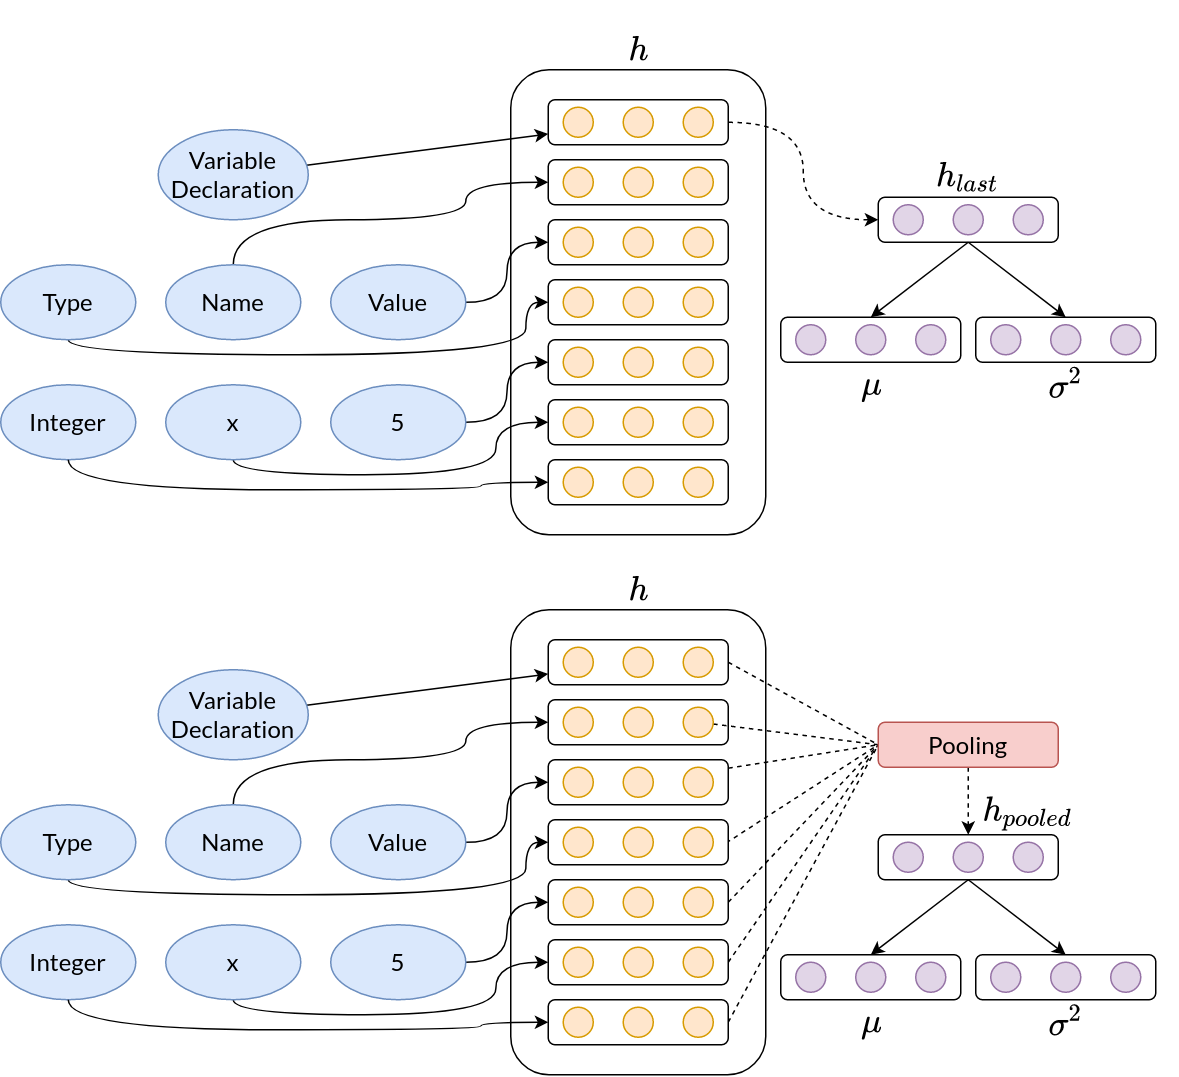
\includegraphics[width=\linewidth]{pooling.png}
    \caption[RNN pooling]{\textbf{Top}: Typical architecture of encoder model of VAE in which only the last hidden state from the RNN is used to compute the mean $u$ and variance $\sigma^2$. \textbf{Bottom}: A pooling method to aggregate the hidden states from the RNN to compute the mean $u$ and variance $\sigma^2$.}
    \label{fig:pooling}
\end{figure}




\paragraph{Neural attention} Tree-LSTM layers are followed by an attention layer. 
The node importance calculation is based on \cite{winata2018attention}, and updates the hidden states as follows:
% Isn't this also \odot rather than \cdot?
\begin{align}
    \mathbf{h}_{at} = \mathbf{h} \cdot tanh(\mathbf{W} \cdot \mathbf{h} + \mathbf{b})
\end{align}

Here, $h$ denotes the hidden states of the last Tree-LSTM layer. This additional layer allows the network to prioritize nodes that contain the most information. 


\paragraph{Pooling} 
The last step in the architecture is the pooling layer responsible for compressing the sequence of $h_{at}$ into a fixed size vector. 
We rejected a common \cite{fabius2015variational} approach of only taking the last hidden state of the RNN as the input to the decoder due to the long-term memory loss problem \cite{kao2020comparison} and use max pooling instead, see figure \ref{fig:pooling}.



\paragraph{Sampling latent code} The pooled vector is then used to compute the mean and variance of the approximate posterior to sample a latent code $z$ with the help of the reparametrization trick \cite{kingma2013auto}. The mean and variance are computed using linear layers that learn a set of weights and biases. 


\newpage
\subsection{Decoder}
The goal of the decoder network is to reconstruct a given input as accurately as possible, given the latent code produced by the encoder. 

\paragraph{Tree decoding} We use the same tree structure for decoding as we used for encoding. 
Having a reversed order of the input sequence compared to the reconstructed sequence has been shown in \cite{fabius2015variational} to improve the performance of the model. 
We employ this technique in our model, which means that since our encoder processes trees bottom-up, the decoder will produce trees top-down. 
The idea here is that the first steps of decoding the tree are more related to the latent space than the last steps.



A method called the doubly-recurrent neural network (DRNN) \cite{alvarezmelis2017tree} allows for top-down tree generation from an encoded vector representation. This method operates solely on the vector representation and does not require that either the tree structure or the nodes are given. The DRNN is based on two recurrent neural networks, breadth and depth-wise, to model ancestral and fraternal information flow. For some node $y$ with parent $pa(y)$ and previous sibling $s(y)$, the ancestral and fraternal hidden states are computed as follows:

\begin{align}
    \mathbf{h}_a^y &= rnn_a(\mathbf{h}_a^{pa(y)}, \mathbf{i}^{pa(y)}) \\ \label{eq:ancestral_update}
    \mathbf{h}_f^y &= rnn_f(\mathbf{h}_f^{s(y)}, \mathbf{i}^{s(y)}) 
\end{align}

Where $rnn_a$, $rnn_f$ are functions that apply one step of the ancestral and fraternal RNNs, respectively. Furthermore, $\mathbf{i}^{pa(y)}$, $\mathbf{i}^{s(y)}$ are the input values (label vectors) of the parent and previous sibling respectively. After the ancestral and fraternal states of $y$ have been computed with the observed labels of its parent and previous sibling, these states can be combined to form a predictive hidden state:

\begin{align}
    \mathbf{h}^y_{pred} = \tanh\left((\mathbf{W}_a \cdot \mathbf{h}_a^y + \mathbf{b}_a) + (\mathbf{W}_f \cdot \mathbf{h}_f^y + \mathbf{b}_f)\right)
\end{align}

Where the operations applied to $\mathbf{h}_a^y$, $\mathbf{h}_f^y$ are linear layers with learnable weights and biases. This combined state then contains information about the nodes' surroundings in the tree.



For each node in the tree, the model needs to decide whether it has offspring and whether it has any successor siblings. We can use the predictive hidden state of a node $\mathbf{h}^y_{pred}$, with a linear layer and a sigmoid activation to compute the probability for offspring and successor siblings as:

\begin{align}
    p_a^y &= \sigma(\mathbf{W}_{pa} \cdot \mathbf{h}_{pred}^y + \mathbf{b}_{pa}) \label{eq:prob_ancestral} \\
    p_f^y &= \sigma(\mathbf{W}_{pf} \cdot \mathbf{h}_{pred}^y + \mathbf{b}_{pf})\label{eq:prob_fraternal}
\end{align}

During training, we use the actual values for whether a node has children and successor siblings. 
During inference, we can either greedily choose any confidence level to continue creating offspring and succeeding siblings by checking whether the probability is above some threshold or sample this choice. 



Besides topological predictions, the model should also predict the label of each token. Again the predictive hidden state can be used for label prediction as follows:

\begin{align}
    \mathbf{o}^y =  softmax\left(\mathbf{W}_o \cdot \mathbf{h}_{pred}^y + \mathbf{b}_{o}\right) \label{eq:label_pred}
\end{align}


\paragraph{Tree decoding optimizations} Now that we have the basic DRNN model \cite{alvarezmelis2017tree} in place to generate a tree from scratch using a latent vector, we can optimize it for our use case. 



The first issue is the possibly infinitely large vocabulary that source code allows. Since progam behavior is invariant to identifier replacement we map each unique identifier to a reusable ID \cite{tufano2019learning} and treat the prediction of identifiers as a clustering problem between declarations and references. We use the predictive hidden states of the nodes to learn relationships between declarations and references.  



The model can keep track of a list of the declared identifiers while generating an AST. Each time a new identifier is declared, a new reusable ID is added to the list. Then for each reference, we can compute the similarity to each of the declared identifiers using some similarity function and predict the most similar identifier. We can keep track of what type of node we are currently trying to predict due to the AST structure and because we have access to the parent node label, i.e., the parent node indicates whether the child node is a declaration or reference. Let $D$ be the set of currently declared identifier nodes and $y$ be the current reference node we are trying to predict, the most similar declared identifier can be computed as follows:

\begin{align}
    \mathbf{s}^{yz} &= similarity(\mathbf{W}_c \cdot \mathbf{h}^y_{pred} + \mathbf{b}_c,  \mathbf{W}_c \cdot \mathbf{h}^z_{pred} + \mathbf{b}_c) \\
    \mathbf{r}^y &= \min_{z \in D}(\mathbf{s}^{yz})
\end{align}



We have a similar problem for literal tokens; developers can use an almost infinitely large number of unique literals in source code. However, in contrast to identifier tokens, literal tokens influence the functionality of a program. Therefore, to assure that generated programs are still compile-able, we cannot remap the literal tokens to reduce the token count. For example, we cannot map rarely used literals to special unknown tokens, as unknown tokens create compiler errors. Instead, we can employ adaptive softmax \cite{grave2017efficient} to use a vocabulary consisting of many unique literal tokens without a considerable increase in computational complexity.



We have identifiers and literals as token categories already, but we can also categorize the leftover tokens into the following categories:

\begin{itemize}
    \item \textbf{Reserved tokens:} for, if, while, ...
    \item \textbf{Types:} int, long, string, ...
    \item \textbf{Built in function names:} printf, scanf, push, ...
\end{itemize}



In total, the five categories cover all the different tokens of the programming language (at least for C++). The reason for splitting up the leftover tokens into more categories is to predict these categories separately based on their parent node. For example, this ensures that we do not input a type-token in the tree, where there should be a reserved token. The categorization improves the compilation rate of the generated programs by allowing the model only to predict tokens of the correct token category. The tree-structured representation during decoding allows us to use this optimization technique. For the reserved tokens, type, and built-in function names, equation \ref{eq:label_pred} is used for label prediction, as there is only a limited number of unique tokens in these categories. 



To allow for the categorized label predictions, we need to add one more element to the DRNN model. 
An essential aspect of the tree structure is that identifiers, built-in function names, and literals occur in the leaves of the trees. 
Hence if a node has offspring, the category of the current node must be a reserved token. 
However, if a node has no offspring, it can be either of the categories, and we need to somehow decide which category to predict a label for. Note that a reserved token can also be on a leaf node on the tree. For example, consider an empty return statement. For that reason, similar to the topology predictions, we have the model predict whether a node is of the reserved token category or not. This prediction  is computed in the same way as the topology predictions using the predictive hidden state of the node as follows: 

\begin{align}
    p_r^y &= \sigma(\mathbf{W}_{pr} \cdot \mathbf{h}_{pred}^y + \mathbf{b}_{pr}) \label{eq:res_pred}
\end{align}



\paragraph{Add gate} The DRNN model has a large flaw, where it is not able to differentiate between paths with the same prefix. For example, consider the situation depicted in figure \ref{fig:treeAddGate}, where we have two function declarations named `add' and `main'. Due to the information flow downwards, both name nodes have the same hidden state and the model is not able to distinguish the leaf nodes and will therefore predict the same label for both. This issue is depicted in the left image of figure \ref{fig:treeAddGate}. To solve this issue, we would like to incorporate the fraternal states in the downwards flow for the model to learn to differentiate the paths downwards. Hence we would like to revise eq. \ref{eq:ancestral_update}, where we take inspiration from the LSTM model and apply the idea of the add gate to our ancestral update formula as follows:

\begin{align}
    &\mathbf{m}_f^y = \sigma(\mathbf{W}_m \cdot \mathbf{h}_f^y + \mathbf{b}_m)\\
    &\mathbf{a}_f^y = tanh(\mathbf{W}_a \cdot \mathbf{h}_f^y + \mathbf{b}_a)\\
    &\mathbf{h}_a^y = \mathbf{h}_a^y + (\mathbf{a}_f * \mathbf{m}_f)
\end{align}

This update to the fraternal state is applied after predicting the label for node $y$, which is depicted in the right image of figure \ref{fig:treeAddGate}. Here, $a_f^y$ is the value of the transformation on the previous sibling state that should be added to the parent state, where the $tanh$ transforms it between -1 and +1 to mitigate exploding gradients. Furthermore, $m_f^y$ decides which elements should be added using a sigmoid function that outputs values between 0 and 1. By multiplying $a_f^y$ with $m_f^y$, the model can learn to decide what and how much to add from the previous sibling state to each parent state's element to help predict the next steps of the tree.


\begin{figure}[ht!]
    \centering
    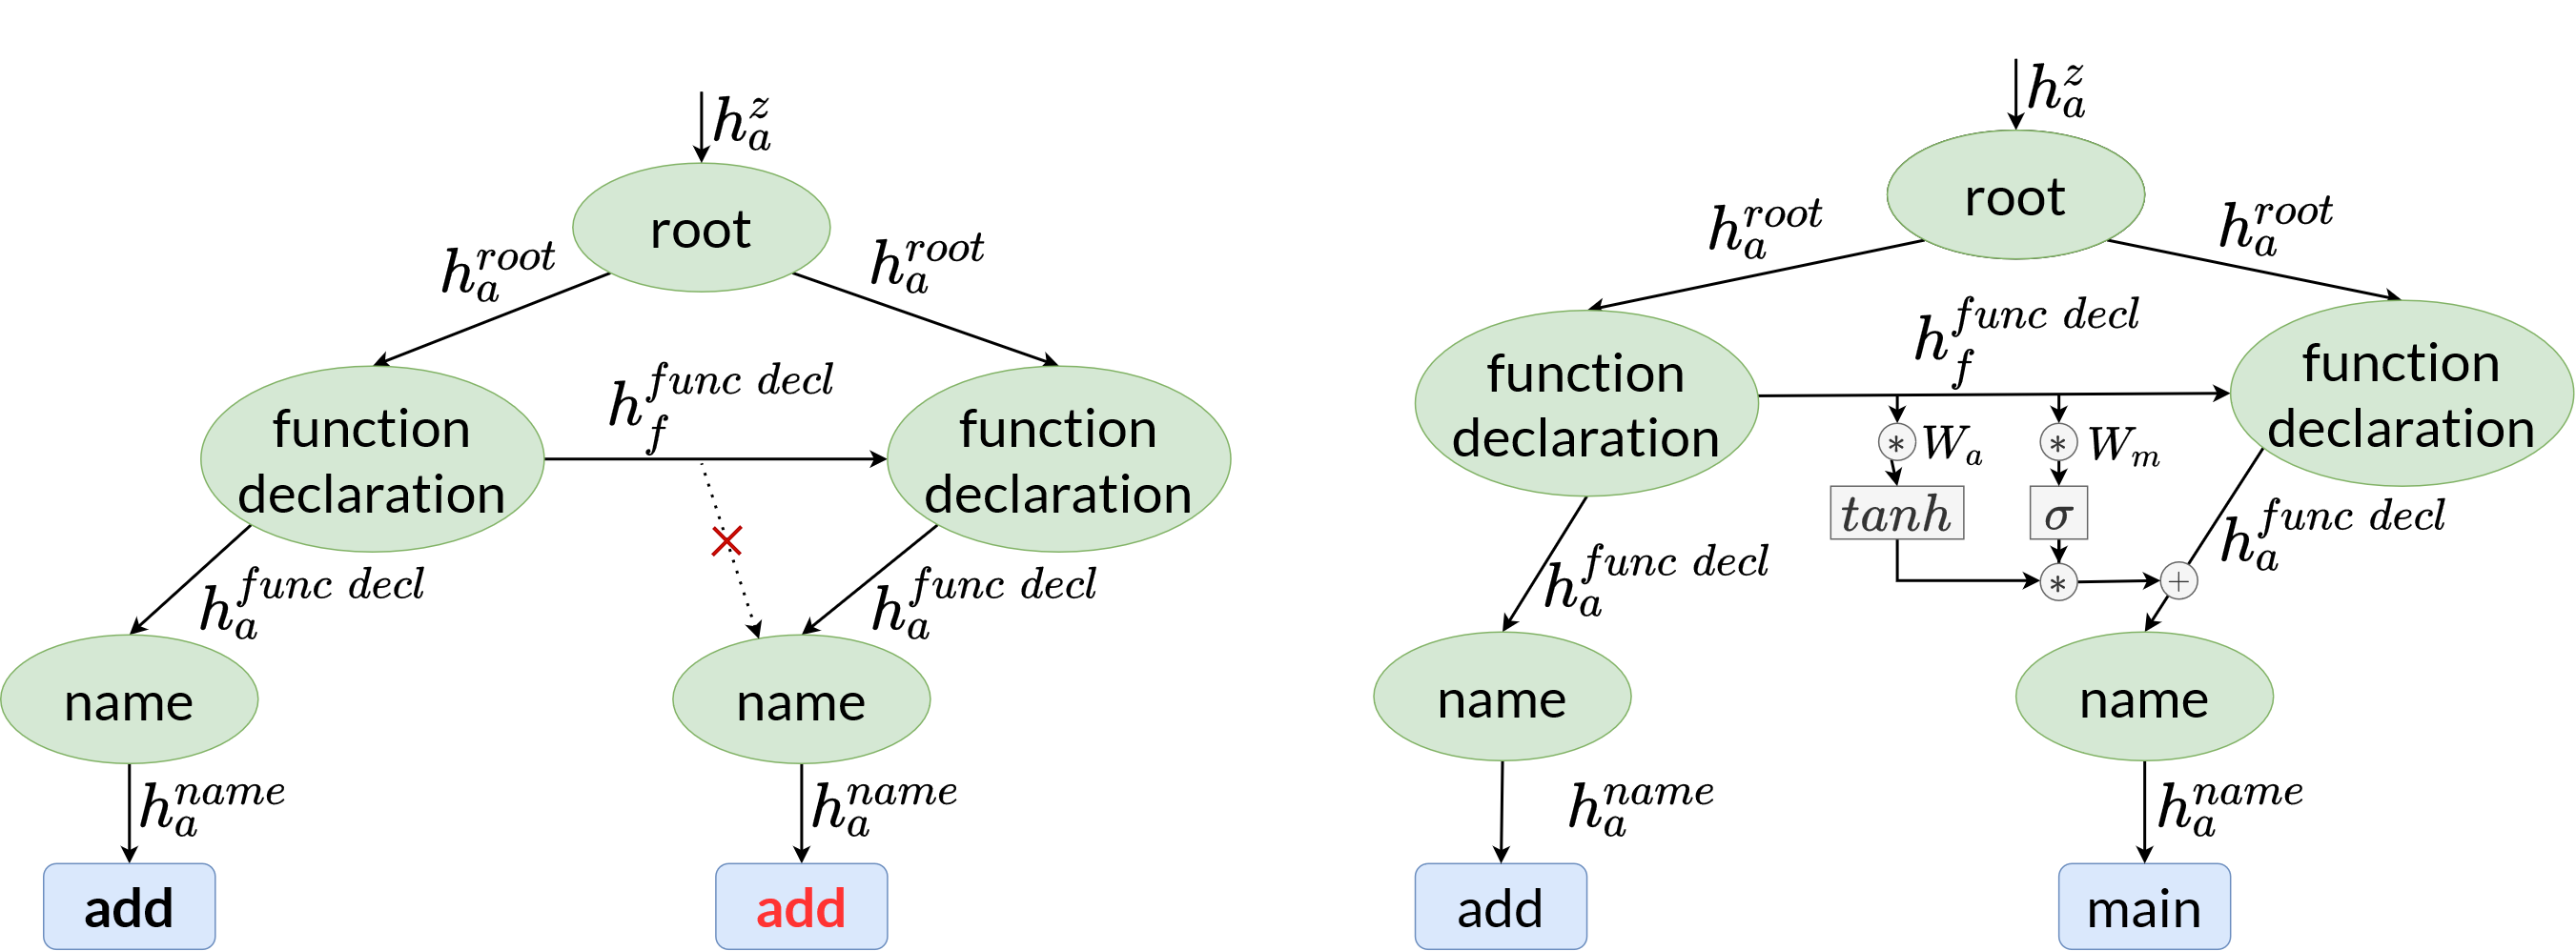
\includegraphics[width=\linewidth]{TreeAddGate.png}
    \caption{DRNN expanded with an add gate to allow for information flow from previous siblings downwards}
    \label{fig:treeAddGate}
\end{figure}

% TODO: say that the model allows for batching
% This is actually an advantage we have
%\subsection{Batching}
%We employ batching in the encoder and decoder to allow for efficient computation on GPUs. In the encoder, the computation of a node in the tree is dependent on all of its children. Therefore, the tree is processed bottom-up, and the trees can be processed in layers. For the decoder process, each node has two dependencies: the parent node and the previous sibling. Here, we process the tree top-down and from left to right at the same time. Note that each first child\footnote{With the first child, we refer to the left-most child} does not have a previous sibling. Therefore, each time a node is processed, its first child node can be computed in the next step. Moreover, because sibling nodes have the same parent, the direct successor sibling may also be computed in the next step. Hence, after processing a node, assuming the node has any offspring and successor siblings, the first child and successor sibling can be computed in the next time step.

% 

% For identifier tokens, the decoder model deviates slightly from this batching process. Because we treat the prediction of the identifier tokens as a clustering problem, we need the predictive hidden states of all the already declared identifiers when predicting a reference. A reference to an identifier may be processed before the declaration of a variable in the current setup. However, for predicting the correct label of a reference, we need to process its declaration first. Therefore, we process the identifier nodes separately, only after all other nodes have been processed. The order in which the identifier nodes are processed is from left to right within a tree, node by node. We ensure that declarations are always processed before their references by processing the identifier nodes from left to right. We parallelize this operation again across multiple trees. An example of the process is depicted in figure \ref{:treeBatchingIdentifiers}.
\newpage
\subsection{Optimization}

\paragraph{Mitigating KL vanishing}
KL vanishing is a common issue when dealing with VAEs with a decoder parameterized by an auto-regressive model.
We mitigate it vanishing using cyclical KL cost annealing \cite{fu2019cyclical}. Furthermore, we apply pooling to the hidden states of the RNN network in the encoder. Long \textit{et al.} \cite{long2019preventing} show this pooling method can effectively prevent the posterior collapse issue. 

\paragraph{Loss function}
Predicting whether a node has offspring and successor siblings are binary choices, so we can use binary cross-entropy to compute the loss for predicting the topology of the AST. 
Let $a^y$, $f^y$ represent the actual values of having offspring and successor siblings for node $y$, the topological losses for this node are then computed as follows:

\begin{align}
    \mathcal{L}_{a}(y) = - a^y \cdot \log(p^y_a) + (1 - a^y) \cdot \log(1 - p^y_a) \\
    \mathcal{L}_{f}(y) = - f^y \cdot \log(p^y_f) + (1 - f^y) \cdot \log(1 - p^y_f)
\end{align}

\noindent where $\mathcal{L}_{a}$, $\mathcal{L}_{f}$ denote the ancestral and fraternal loss respectively. Because the reserved token category prediction (eq. \ref{eq:res_pred}) is so similar to the topological predictions, the loss for that component can be defined in a similar fashion:

\begin{align}
    \mathcal{L}_{r}(y) = - r^y \cdot \log(p^y_r) + (1 - r^y) \cdot \log(1 - p^y_r)
\end{align}

\noindent where we define $r^y$ to represent the actual value of node $y$ being in the reserved token category. 



Label prediction is a classification problem for all label categories, except the identifiers.
Hence, we can compute the cross entropy loss (or negative log likelihood):

\begin{align}
    \mathcal{L}_{l}(y) = - \log(\mathbf{o}^y[l^y])
\end{align}

\noindent where we assume that $l^y$ is the index of the true label, and hence $\mathbf{o}^y[l^y]$ retrieves the softmax value at the index of the correct class. 

Lastly, since predicting the labels of identifier (reference) tokens is treated as a clustering problem, we can use triplet loss \cite{chechik2010large}. 
To compute the loss of a reference node $y$, we select the true declaration node $z$ and sample a negative declaration node $x$; the loss is then defined as follows:

\begin{align}
    \mathcal{L}_i(y)=\max(\mathbf{s}^{yx} - \mathbf{s}^{yz},0)
\end{align}

\noindent We can then combine all of the separate components to form a single reconstruction loss function for a node:

\begin{small}
\begin{align}
   \mathcal{L}_{rec}(y) = 
\begin{cases}
    \mathcal{L}_{a}(y) + \mathcal{L}_{f}(y) + \mathcal{L}_{r}(y),& \text{if } y \text{ is a declaration} \\
    \mathcal{L}_{a}(y) + \mathcal{L}_{f}(y) + \mathcal{L}_{r}(y) + \mathcal{L}_{i}(y),& \text{if } y \text{ is a reference} \\
    \mathcal{L}_{a}(y) + \mathcal{L}_{f}(y) + \mathcal{L}_{r}(y) + \mathcal{L}_{l}(y),& \text{otherwise}
\end{cases}
\end{align}
\end{small}

Because the loss is decoupled, this allows us to weigh the objectives differently to emphasize, for example, topology or label prediction accuracy. We leave experimenting with different weights for objectives as future work. 

The total loss function, combining the KL divergence, KL weight $w$ and reconstruction loss becomes:

\begin{align}
    \mathcal{L}(N) = \mathcal{L}_{tot\_rec}(N) = \sum_{y \in N}\mathcal{L}_{rec}(y) - w \cdot D_{KL}\left(Q(z|N)||P(N)\right)
\end{align}

During training, we perform teacher forcing, technique that is commonly used with sequence generation.

\begin{figure*}[ht!]
    \centering
    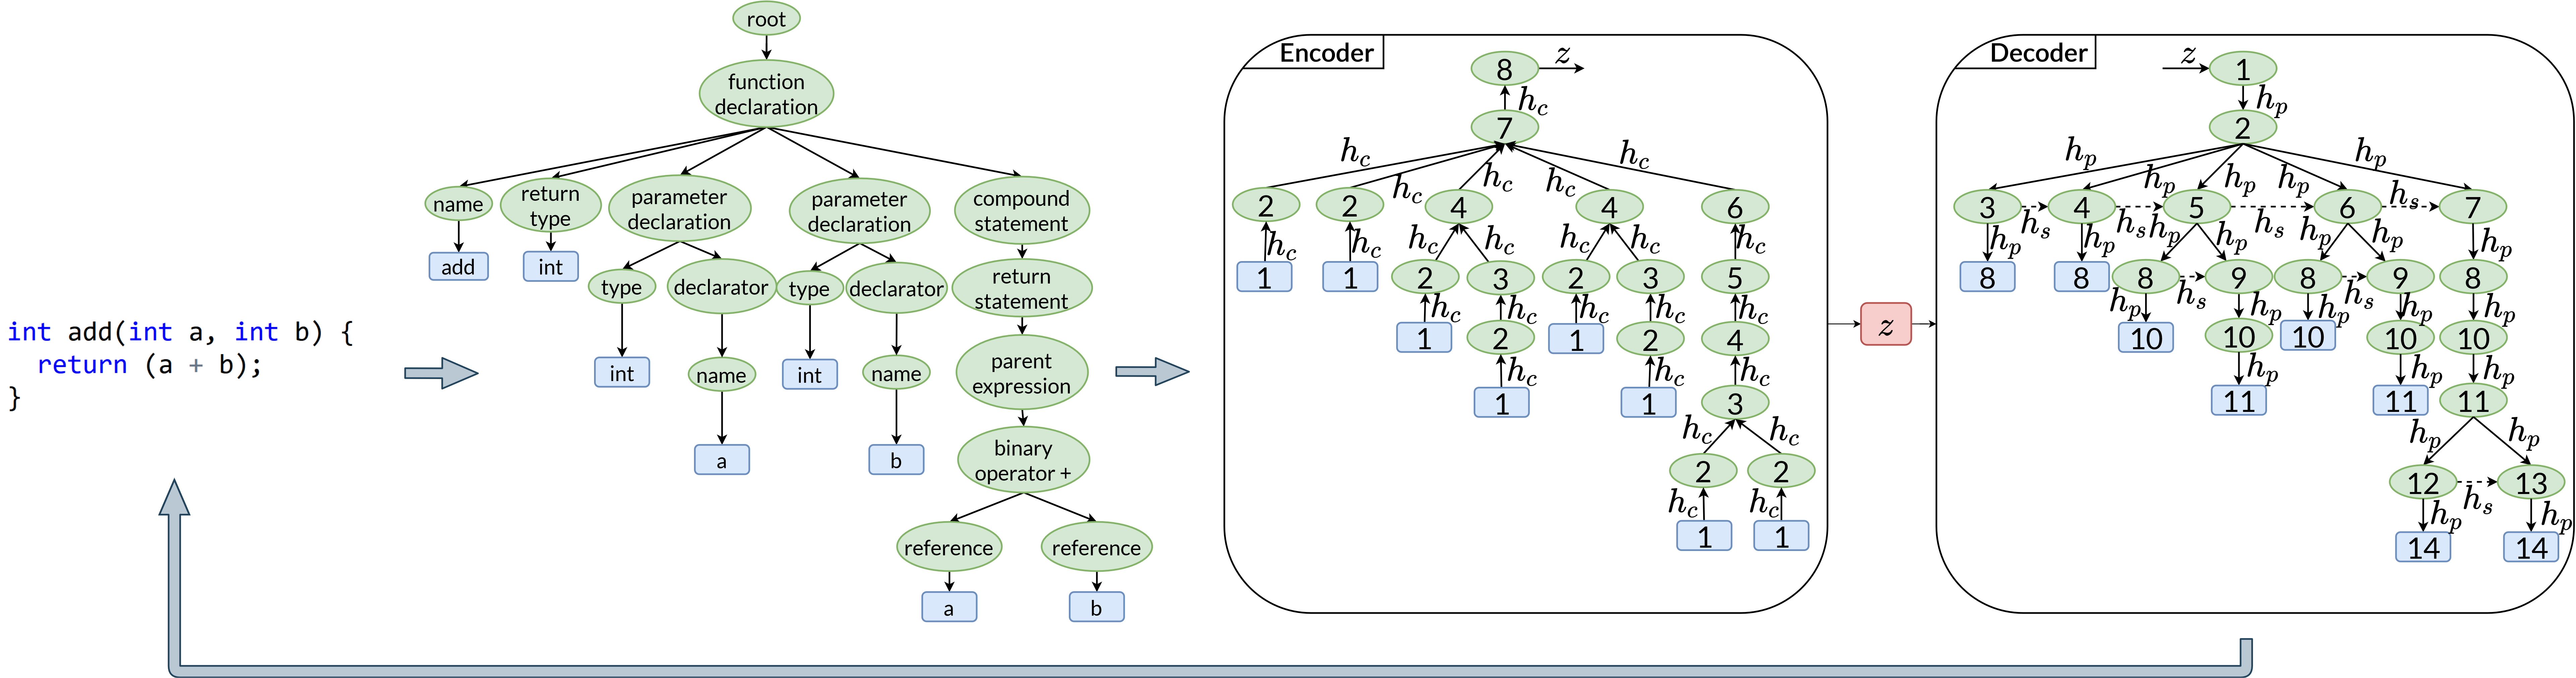
\includegraphics[width=\linewidth]{tree2treeLSTM2.png}
    \caption[Tree2Tree model high-level overview]{Tree to tree autoencoder overview. \textbf{First Fig.}: The piece of code considered. \textbf{Second Fig.}: The piece of code parsed to an AST tree format. \textbf{Third Fig.}: The order in which the encoder module encodes the tree structure bottom-up. Here, $h_c$ indicates the hidden state that travels from a child to a parent. \textbf{Fourth Fig.}: The order in which the decoder module decodes the tree structure top-down. Here, $h_p$ indicates the hidden state that travels from a parent to a child, and $h_s$ indicates the hidden state that travels from a node to its successor sibling.}
    \label{fig:tree2treeVAE}
\end{figure*}

\newpage
\section{Evaluation}
\label{evaluation}

\paragraph{Dataset}
We train and evaluate our model on a dataset of programs from code competition websites. Programs from these platforms exhibit a few qualities that are suitable for program synthesis. The programs are tested and known to be syntactically correct and compile-able, and they are standalone code fragments and do not depend on any code that is not built into the programming language. The dataset consists of almost two million C++ programs across 148 competitions divided over 904 problems. 

The programs in the data set are generally structured to contain a main function, standard input and output stream elements, computation and memory optimizations, and possibly some other elements such as helper functions/classes. Due to this general structure, the programs tend to overlap in their content, in contrast to, for example, natural language sentences. 

\paragraph{Baseline}
Our method is compared to a baseline inspired by autoencoders used for text generation in natural language. We can also evaluate how well these models generalize to source code synthesis by taking inspiration from natural language models. The model architecture is inspired from \cite{bowman2015generating}. In this architecture, both the encoder and decoder networks contain single-layer recurrent neural networks. A Gaussian prior is used for the regularization of the latent space. The model operates on the original sequences of source code and decodes the latent vector back to the source code without an intermediate structured representation. Therefore we refer to the baseline model as the Sequence-to-Sequence (Seq2Seq) model, and the architecture is depicted in figure \ref{fig:seq2seq}.

\begin{figure*}[ht!]
    \centering
    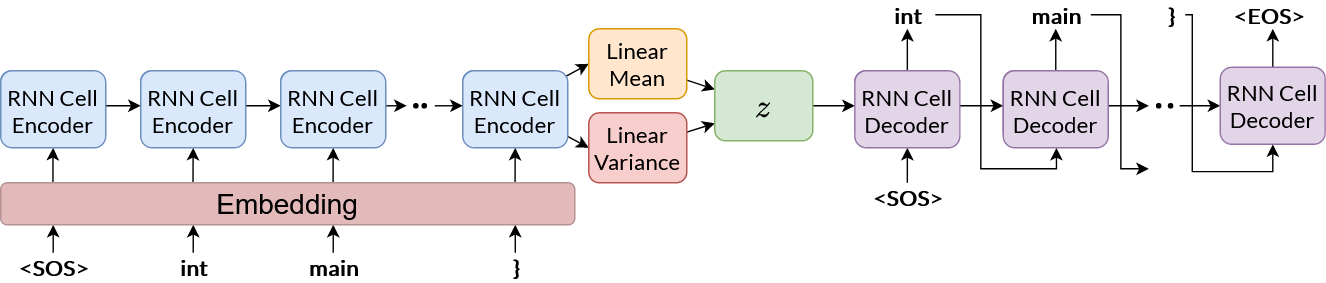
\includegraphics[width=0.8\linewidth]{seq2seq.png}
    \caption{The architecture of the Seq2Seq model}
    \label{fig:seq2seq}
\end{figure*}

Similar to our proposed autoencoder model, we employ methods to mitigate KL-vanishing. Again, we use cyclic KL annealing \cite{fu2019cyclical}, and we combine this with a technique called word dropout \cite{bowman2015generating} to weaken the decoder.

We use three-layered LSTMs in the encoder and decoder with a recurrent dropout rate of 20\% to reduce over-fitting. The embedding layer is initialized with Glove wiki gigaword 50 \cite{pennington2014glove} embedding. We train the model using the Adam optimizer \cite{kingma2014adam} with a learning rate of $1e-3$ and 10 epochs with early stopping and a patience of 3. We train and run the experiments on GPUs with a batch size set to 32.

\paragraph{Reconstruction results}\label{sec:recon-results}
First of all, we look at how accurately the autoencoders can reconstruct programs. We use a separate test split containing around 60.000 samples of our data set to evaluate this and use these samples as input for the autoencoders. 



We compute BLEU scores \cite{papineni2002bleu} for both models on the original representation of the source code to obtain comparable results, i.e., we do not use the tree representation. The Tree2Tree model thus has an extra step to use the data parser to transform the tree representation back to source code. This extra step is disadvantageous for the Tree2Tree model as it may introduce some errors due to imperfections in the parsing process. The BLEU scores are then computed on each token in a program: keywords, identifiers, operators, and special symbols such as semicolons or braces. We report on the cumulative BLEU-1 through BLEU-4 scores to indicate the overlap between original and reconstructed programs. Furthermore, we present the percentage of reconstructed programs that compile to indicate how well the models have learned the programming language's syntax. We experiment with different combinations of latent sizes $l$ and hidden RNN dimensions $h$:  ($l$:10,  $h$:50), ($l$:50, $h$:100), ($l$:100, $h$:200), ($l$:150, $h$:300), ($l$:300, $h$:500), ($l$:500, $h$:800), ($l$:800, $h$:1200).



We use greedy decoding in reconstruction experiments (table table \ref{tab:rec_results}) to maximize accuracy. In contrast, sampling is used in generation tasks where diversity of candidates can be helpful.

\begin{table}[ht!]
\centering
% A table with adjusted row and column spacings
% \setlength sets the horizontal (column) spacing
% \arraystretch sets the vertical (row) spacing
\begingroup
\setlength{\tabcolsep}{3pt} % Default value: 6pt
\renewcommand{\arraystretch}{1.4} % Default value: 1
\begin{tabular}{cccccccc}
 & \textbf{Latent} & \textbf{BLEU-1} & \textbf{BLEU-2} & \textbf{BLEU-3} & \textbf{BLEU-4} & \textbf{Compiles}\\ \hline
\multirow{7}{*}{Seq}    &   10   &  0.037   &    0.024     &     0.017     &    0.013       &    0.000\%   \\
                            &   50   &      0.085    &      0.061         &         0.047      &    0.037       &       42.467\%      \\
                            &   100   &  0.295   &      0.225     &     0.176      &    0.141       &   65.808\%               \\
                            &   150   &     0.278  & 0.211          & 0.165          & 0.131          &  66.971\%              \\
                            &   300   & 0.346                     &  0.262                        &     0.203                     &     0.161                     & 60.651\% \\   
                            &   500   &  0.421                   &      0.332                    &         0.263                 &      0.211                    &  90.329\% \\
                            &   800   &  0.429                   &      0.329                    &         0.253                 &      0.195                    &  \textbf{91.784\%} \\\hline
\multirow{7}{*}{Tree}  &   10   &  0.445  &    0.339     &     0.260     &     0.202      &   28.375\%    \\
                        &   50   &     0.417    &      0.317    &       0.242    & 0.189  &  23.256\% \\
                            &   100   &     0.423      &      0.323     &     0.251      &  0.200 &      30.429\%     \\
                            &   150   & \textbf{0.486} &     \textbf{0.382}    &  \textbf{0.302}     &      \textbf{0.243}    &   35.419\%           \\
                            &   300   &   0.457                 &     0.342                &      0.260                &     0.202                   & 35.054\% \\   
                            &   500   &     0.398                &      0.301             & 0.230      &             0.178             &            36.022\%      \\
                             &   800   &     0.258                &      0.182             & 0.131      &             0.096             &     2.358\%      \\
\end{tabular}
\endgroup
\caption{Reconstruction results.}
\label{tab:rec_results}
\end{table}

The results listed in table \ref{tab:rec_results} show the superiority of the Tree2Tree model in terms of reconstruction capability (BLEU scores), especially for smaller latent sizes. The reconstruction scores of the Tree2Tree model of latent size 150 outperform all the Seq2Seq models up to latent size 800. In contrast, the Seq2Seq models show to perform much better at constructing compile-able programs, which improves with the model's size, to nearly 100\%. This is a surprising result, which is investigated in more detail in section \ref{evaluation}.

 


An interesting result is that the performance of the models does not necessarily increase with the size of the model. Especially for the Tree2Tree models, we see that after latent size 150, the models' performance decreases. In general, one would expect that the model would perform better with an increase in latent size, allowing more information flow between the encoder and decoder. We hypothesize that, because not only the latent size increases but also the number of hidden units in the auto-regressive models, the models experience KL vanishing. Due to the increasing hidden units, the auto-regressive models become stronger and may depend more on their predictions, ignoring information from the latent vector. In turn, the reconstruction performance vastly decreases. Confirmation of this hypothesis is left as a venue for future work.



Next, we would like to experiment on how different input sizes affect the performance of both models. Due to the tree-structured representation used by the Tree2Tree model, the size of the sequences that the RNNs process scale proportionally to the width and depth of the tree. The Seq2Seq model, on the other hand, processes sequences left to right, hence the number of computations of the RNNs scale directly with the sequence length. 



To evaluate the performance on different sized inputs, we split the test data set into three subsets. A small, medium and large subset with the following properties:

\begin{itemize}
    \item \textbf{small subset}: maximum of 250 tokens
    \item \textbf{medium subset}: between 251 and 500 tokens
    \item \textbf{large subset}: between 501 and 750 tokens
\end{itemize}

 

We compute the BLEU scores and compilation percentage again using greedy decoding on the smaller subsets for the best performing Seq2Seq and Tree2Tree models, based on the results of table \ref{tab:rec_results}. Here, performance is based on the combination of BLEU-4 and compilation percentage. For Seq2Seq, this is the model with latent size 500. Similarly, for Tree2Tree, this is the model with latent size 150. The results are depicted in table \ref{tab:rec_results_inp_sizes}.



%150 latent t2t lr 0.001 large test set (> 500, <= 750): bleu1 0.317, bleu2 0.236, bleu3 0.177, bleu4 0.134, compiles 5.001

%150 latent t2t lr 0.001 medium test set (> 250, <= 500): bleu1 0.468, bleu2 0.364, bleu3 0.284, bleu4 0.225, compiles 21.241


\begin{table}[ht!]
\centering
% A table with adjusted row and column spacings
% \setlength sets the horizontal (column) spacing
% \arraystretch sets the vertical (row) spacing
\begingroup
\setlength{\tabcolsep}{3pt} % Default value: 6pt
\renewcommand{\arraystretch}{1.4} % Default value: 1
\begin{tabular}{clccccc}
 & \textbf{Input} & \textbf{BLEU-1} & \textbf{BLEU-2} & \textbf{BLEU-3} & \textbf{BLEU-4} & \textbf{Compiles}\\ \hline
\multirow{3}{*}{Seq}    &   small   &   0.513  &    0.403    &      0.321    &  0.258      &  95.334\%     \\
                            &   medium   &  0.306      &    0.244        &      0.192     & 0.153      & 86.812\% \\
                            &   large   &    0.196   &      0.157   &   0.123       &   0.096       &  87.971\% \\ \hline
\multirow{3}{*}{Tree}  &   small   &   0.633  &    0.516     &     0.424     &     0.355      &  59.022\%                \\
                            &   medium   &   0.478  &   0.371        &          0.289 &     0.229   & 21.241\%            \\
                            &   large   &  0.324 &      0.242  & 0.181    &    0.138     &    5.001\%         \\ 
\end{tabular}
\endgroup
\caption{Reconstruction results of the best models on different input sizes.}
\label{tab:rec_results_inp_sizes}
\end{table}



From table \ref{tab:rec_results_inp_sizes} we can observe that both models follow the same logical trend: the larger the input size, the lower BLEU-scores and compilation percentages. For the Tree2Tree model, the BLEU scores for the medium subset seem to be similar to the BLEU scores on the entire test set, whereas, for the Seq2Seq model, the BLEU scores are much lower on the medium subset. The models seem to be fairly close in terms of performance degradation from small to large program sizes. For example, we can measure performance degradation for the large versus small subset by dividing the BLEU-4 scores on the large set by the BLEU-4 score on the small set. For the Seq2Seq model, we get a score of $0.372$, and for the Tree2Tree model, we get $0.389$. Similarly, we get $0.593$ and $0.645$ for the Seq2Seq and Tree2Tree model for the medium versus small subset. While the performance degrades less with increasing input sizes for the Tree2Tree model, this difference is insignificant. 



An issue with the aforementioned computation of performance degradation is that it does not correct for elements in programs that are almost always present. For example, each program contains a main function, with standard input and output streams. The models may simply always predict these standard elements of a program and then use the information of the encoder to complete the details of the program. However, this causes the BLEU score to consist of two parts: the score for the prediction of the elements that are always present and the score of what it has learned to predict together with the encoder. The latter is more interesting and shows how much information can be saved in the latent vector. 



Therefore, we apply a correction on the BLEU scores to focus on the prediction based on the information in the latent vector. We compute corrected scores by feeding the decoder with random latent vectors and computing BLEU scores on the subsets of the test data set. Then, we subtract these correction scores from the computed BLEU scores in table \ref{tab:rec_results_inp_sizes}, and take 0 if the result of the subtraction is negative. The corrected BLEU scores including the correction scores are presented in table \ref{tab:corrected_rec_results_inp_sizes}.

\begin{table}[ht!]
\centering
% A table with adjusted row and column spacings
% \setlength sets the horizontal (column) spacing
% \arraystretch sets the vertical (row) spacing
\begingroup
\setlength{\tabcolsep}{3pt} % Default value: 6pt
\renewcommand{\arraystretch}{1.4} % Default value: 1
\resizebox{\linewidth}{!}{%

\begin{tabular}{clccccc}
\textbf{Model}   & \textbf{Input size} & \textbf{BLEU-1} & \textbf{BLEU-2} & \textbf{BLEU-3} & \textbf{BLEU-4} \\ \hline
\multirow{3}{*}{Seq2Seq}    &   small   &   0.072 (0.441)  &    0.077 (0.326)    &  0.075    (0.246)    &  0.070 (0.188)     \\
                            &   medium   & 0.006 (0.300)      &  0.018  (0.226)        &    0.021  (0.171)     & 0.023 (0.130)    \\
                            &   large   &   0.000 (0.213)   &  0.000    (0.166)   & 0.000  (0.128)       &  0.000 (0.099)   \\ \hline
\multirow{3}{*}{Tree2Tree}  &   small   &  0.200 (0.433)  &  0.220  (0.296)     &  0.223   (0.201)     &    0.218 (0.137)        \\
                            &   medium   &  0.148 (0.330)  &  0.147 (0.224)        & 0.146 (0.150) &    0.128 (0.101)        \\
                            &   large   &  0.102 (0.222) &    0.090  (0.152)  &  0.079 (0.102)     &  0.070  (0.068)      &   \\
\end{tabular}%
}
\endgroup
\caption{Corrected BLEU scores of reconstructed results of the best models on different input sizes. (correction scores in parenthesis)}
\label{tab:corrected_rec_results_inp_sizes}
\end{table}



Table \ref{tab:corrected_rec_results_inp_sizes} indicates a large difference in performance degradation between the Seq2Seq model and the Tree2Tree model. A noticeable result is that the corrected BLEU scores for large programs predicted by the Seq2Seq model are 0. Hence, the Seq2Seq model extracts no information from the latent vector at all for large programs. Similarly, for medium-sized programs, little information is transferred between the encoder and decoder. We can again compute the performance degradation scores for the Seq2Seq model, which are $0.280$ and $0.00$ for the medium versus small and large versus small subsets, respectively, on the corrected BLEU-4.



In contrast, the performance degradation is much smaller for the Tree2Tree model:  $0.587$ and $0.321$ for the medium versus small and large versus small subsets, respectively, on the corrected BLEU-4. Hence, the structural nature of the Tree2Tree model scales better to large input sequences than the Seq2Seq model in terms of reconstruction scores, even with a much smaller latent size. 



An interesting observation is that the latent vector conveys relatively little information in terms of BLEU scores. The correction scores make up a large part of the total BLEU scores as presented in table \ref{tab:rec_results_inp_sizes}. Hence, the BLEU scores are largely determined by the models' general knowledge of how C++ programs are built up and not the specific content.

\paragraph{Generative results}
\label{results:gen}
To see how well autoencoders can generate reasonable samples from any point in latent space that conform to the C++ syntax, we sample 1000 random latent vectors from the prior distribution $\mathcal{N}(0, I)$ and input these vectors to the decoder networks. Then, we compute the percentage of generated programs that compiles and is thus also syntactically correct.



We employ two decoding strategies to test the generative capabilities of the models: greedy decoding and sampling. The sampling strategy we apply is a combination of top-$k$, nucleus, and temperature sampling \cite{holtzman2019curious}. We first use temperature sampling to scale the logits to control the shape of the probability distribution. Then, we filter the on the top-$k$ samples, after which we filter tokens on their cumulative probability using nucleus sampling (top-$p$). Lastly, we sample a token from the resulting distribution. The selected sampling hyper-parameters for this experiment are: $k=40$, $p=0.9$, $temperature=0.7$. The results of the experiment are displayed in table \ref{tab:gen_results}.

\begin{table}[ht!]
\centering
% A table with adjusted row and column spacings
% \setlength sets the horizontal (column) spacing
% \arraystretch sets the vertical (row) spacing
\begingroup
\setlength{\tabcolsep}{3pt} % Default value: 6pt
\renewcommand{\arraystretch}{1.4} % Default value: 1
\begin{tabular}{cccc}
\textbf{Model}   & \textbf{Latent size} & \textbf{Greedy search} & \textbf{Sampling} \\ \hline
\multirow{5}{*}{Seq2Seq}    &   10   &  0.0\%   & 0.9\%  \\
                            &   50   &   38.5\%    &  2.9\%   \\
                            &   100   &   62.1\%   &  21.3\%     \\
                            &   150   &   58.0\%  &     23.5\%        \\
                            &   300   &  60.6\%  &  36.8\%   \\   
                            &   500   &  67.5\% & 37.8\% \\
                            &   800   & 78.2\%  & 39.6\% \\\hline
\multirow{5}{*}{Tree2Tree}  &   10   &   29.6\%   & 20.2\% \\
                            &   50    & 22.6\%   &  17.7\%    \\
                            &   100    & 30.3\%  &       22.1\%      \\
                            &   150  &  26.9\%  &   18.8\%     \\
                            &   300  & 23.4\%  & 12.8\%    \\   
                            &   500 & 25.6\%  & 14.4\%\\
                            &   800   &  4.1\% & 6.7\% \\
\end{tabular}
\endgroup
\caption{Generative results compilation percentage.}
\label{tab:gen_results}
\end{table}




The results from table \ref{tab:gen_results} show similar trends as section \ref{sec:recon-results}. The general trend is: the larger the model (in terms of latent size and hidden units), the higher the compilation percentage. Moreover, greedy search during inference gives a higher compilation percentage than sampling. This outcome is not surprising, as, with greedy search, we always pick the label for which the model is most confident. On the other hand, sampling gives a more varied output and may be useful for searching similar programs in a vicinity of the latent space. The trade-off for a more diverse output is thus a lower compilation ratio. 

\newpage
\section{Conclusion}

Our results indicate that Tree Variational Autoencoders have a significant advantage over sequence-to-sequence models in low-dimensional latent spaces, achieving both a higher compilation rate and a higher reconstruction quality.
In higher-dimensional latent spaces seq2seq programs offer a higher compilation rate, but based corrected BLEU scores indicate that this benefit is often achieved by sacrificing reconstruction quality, even to the point of ignoring the input completely.

Overall, our findings support the initial hypothesis that structured autoencoder models are better suited for program synthesis than sequence-to-sequence alternatives.
We believe this result to be a significant step towards an autoencoder-based foundation model for genetic programming and genetic improvement of software.
